\chapter*{Основные теоретические сведения}
\addcontentsline{toc}{chapter}{Основные теоретические сведения}
В ходе лабораторной работы будет использован базовый шаблон так называемого RTL проекта VINC, который может быть создан в IDE Xilinx Vitis и САПР Xilinx Vivado. Шаблон VINC выполняет попарное сложение чисел исходного массива и сохраняет результаты во втором массиве. Проект VINC включает:

Проект ПО хоста, выполняющий инициализацию аппаратного ядра и его тестирование через OpenCL вызовы.

Синтезируемый RTL проект ядра ускорителя на языках Verilog и

SystemVerilog.

Функциональный тест ускорителя VINC на языке SystemVerilog.

Все перечисленные проекты создаются автоматически посредством запуска мастера RTL проектов в IDE Xilinx Vitis, и могут далее модифицироваться как через тот же мастер, так и в ручном режиме в САПР Xilinx Vivado, или обычном текстовом редакторе. Ряд проектных процедур необходимо запустить из консоли ОС Linux.

Проект VINC представляет собой аппаратное устройство, связанное шиной AXI4 MM (Memory mapped) с DDR[i] памятью, и получающее настроечные параметры по интерфейсу AXI4 Lite от программного обеспечения хоста (рисунок \ref{png:func_schema}). В рамках всей системы используется единое 64-х разрядное адресное пространство, в котором формируются адреса на всех AXI4 шинах.

\begin{figure}[H]
	\captionsetup{justification=centering}
	\centering{
		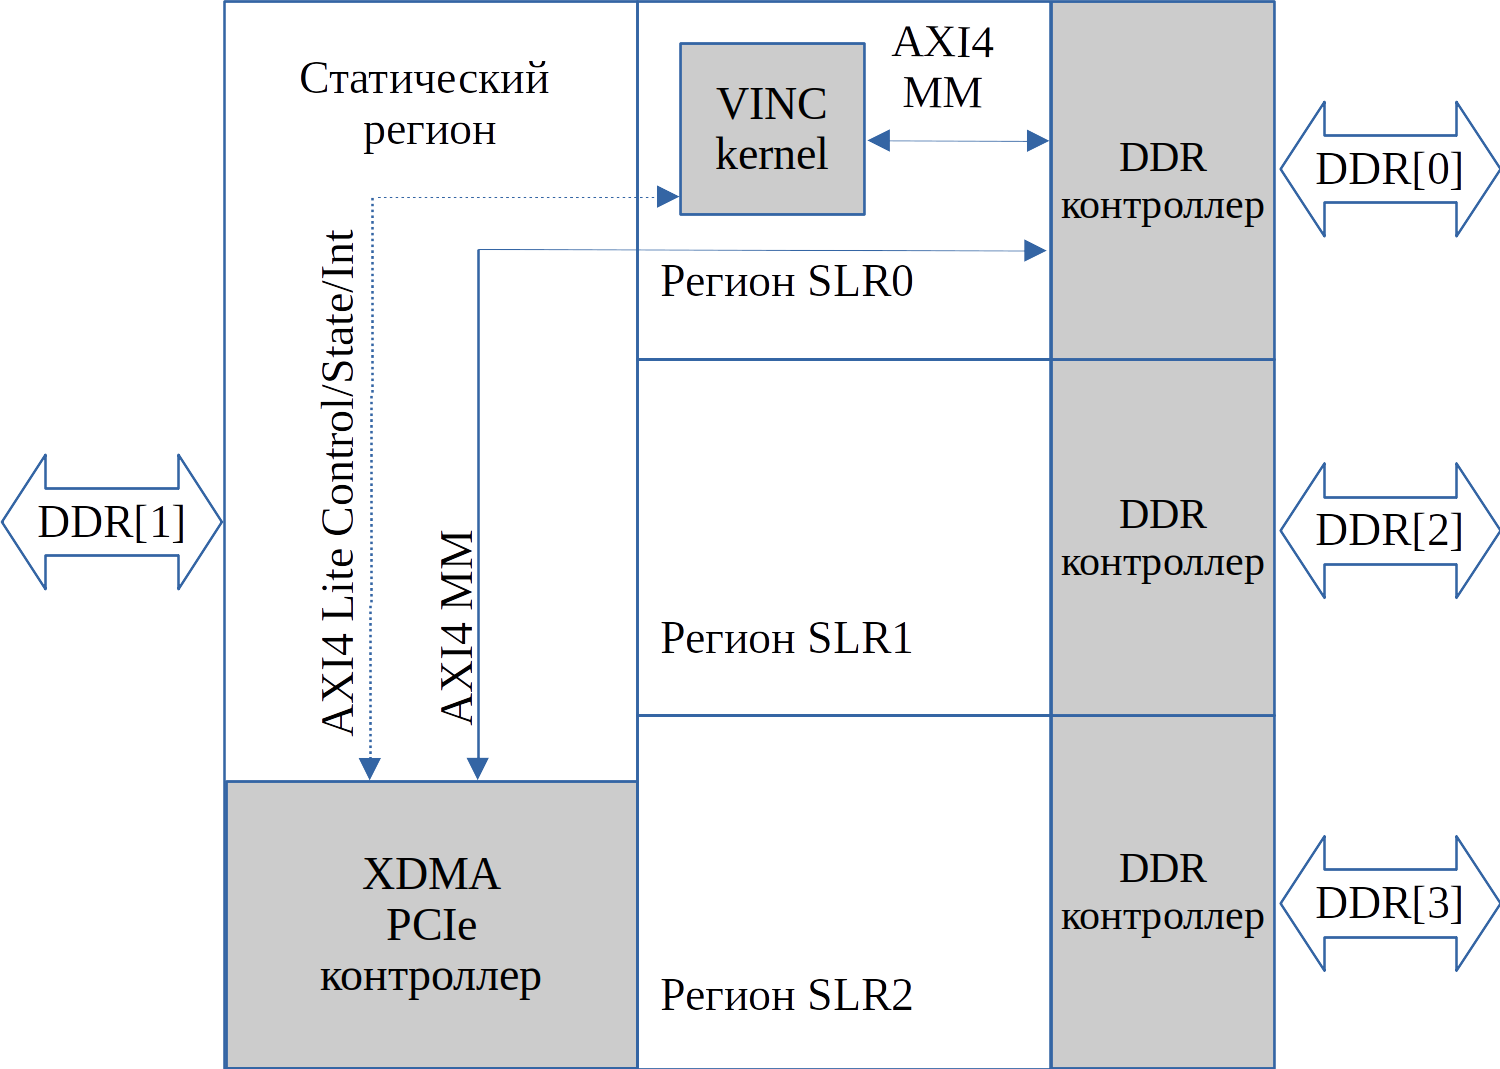
\includegraphics[scale=0.2]{images/func_schema}
		\caption{Размещение проекта на ПЛИС xcu200-fsgd2104-2-e карты Alveo U200}
		\label{png:func_schema}
	}
\end{figure}

В каждой карте U200 имеется возможность подключить ускоритель к любому DDR[i] контроллеру в том регионе, где будет размещен проект. Всего для пользователя доступны 3 динамических региона: SLR0,1,2, для которых выделены каналы локальной памяти DDR[0], DDR[2], DDR[3] соответственно. Вся подключенная память DDR[0..3] доступна со стороны статического региона, в котором размещена аппаратная часть XRT.

Память DDR[1] доступна для использования как в статическом регионе, так и в динамическом регионе SLR1.

Предполагается, что эта память может служить для организации эффективной подсистемы памяти ускорительной карты: буферизации данных, передаваемых между хост-системой и ускорителем.
